\documentclass[10pt]{article}

\usepackage[a4paper, margin=1.4cm]{geometry}
\usepackage[utf8]{inputenc}
\usepackage[T1]{fontenc}
\usepackage{booktabs}
\usepackage{graphicx}
\usepackage{amsmath}
\usepackage{amssymb}
\usepackage{hyperref}
\usepackage{xcolor}
\usepackage{caption}
\usepackage{subcaption}
\usepackage{float}
\usepackage{array}
\usepackage{enumitem}

\captionsetup{font=footnotesize,labelfont=bf,skip=2pt}
\setlist{nosep,leftmargin=1.2em}
\setlength{\abovedisplayskip}{2pt}
\setlength{\belowdisplayskip}{2pt}
\pagestyle{empty}

\hypersetup{colorlinks=true,linkcolor=blue,citecolor=blue,urlcolor=blue}

\begin{document}

\begin{center}
{\large\bfseries Beyond Pixels --- Summary}\\[2pt]
{\small A.\,Chebil \quad H.\,Hennion \quad (proj104 -- T\'el\'ecom Paris) \quad \today}
\end{center}
\vspace{2pt}

\noindent\footnotesize
Multi-label classification of 21 chest pathologies on Open-I (paired image +
report). We study the task by \textbf{text}, then \textbf{image}, then
\textbf{multimodal} fusion. Each report has three sections: \emph{indication}
(clinical question), \emph{findings} (observations), \emph{impression} (conclusion);
labels are derived from \emph{impression} by MeSH matching, giving 21 strongly
imbalanced classes.

% ============================================================
\section{Text (H.\,Hennion)}
% ============================================================
\footnotesize
Goal: \emph{indication\,+\,findings} $\Rightarrow$ labels. A simple
\textbf{TF-IDF\,+\,MLP} ($\sim$1.4k features, one hidden layer) already reaches
macro AUC \textbf{0.864} / micro \textbf{0.927} -- the task is largely \emph{easy
from text}, as the indication often names the pathology. Fine-tuning
\textbf{CXR-BERT-specialized} (progressive unfreezing) lifts this to macro AUC
\textbf{0.972} / micro \textbf{0.987}, macro F1 \textbf{0.734} -- far above any
image model.

\begin{figure}[H]
\centering
\begin{subfigure}{0.49\textwidth}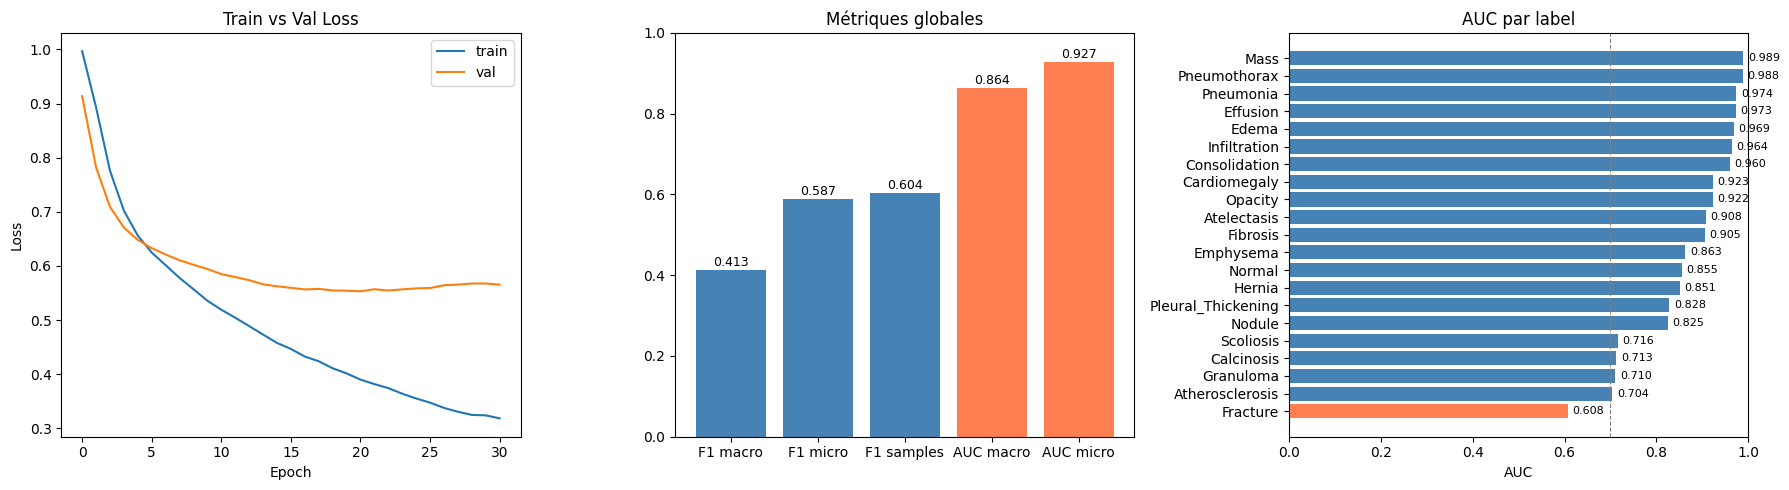
\includegraphics[width=\linewidth]{figures/mlp_tfidf_perf.png}\caption{TF-IDF + MLP baseline (text).}\end{subfigure}
\hfill
\begin{subfigure}{0.49\textwidth}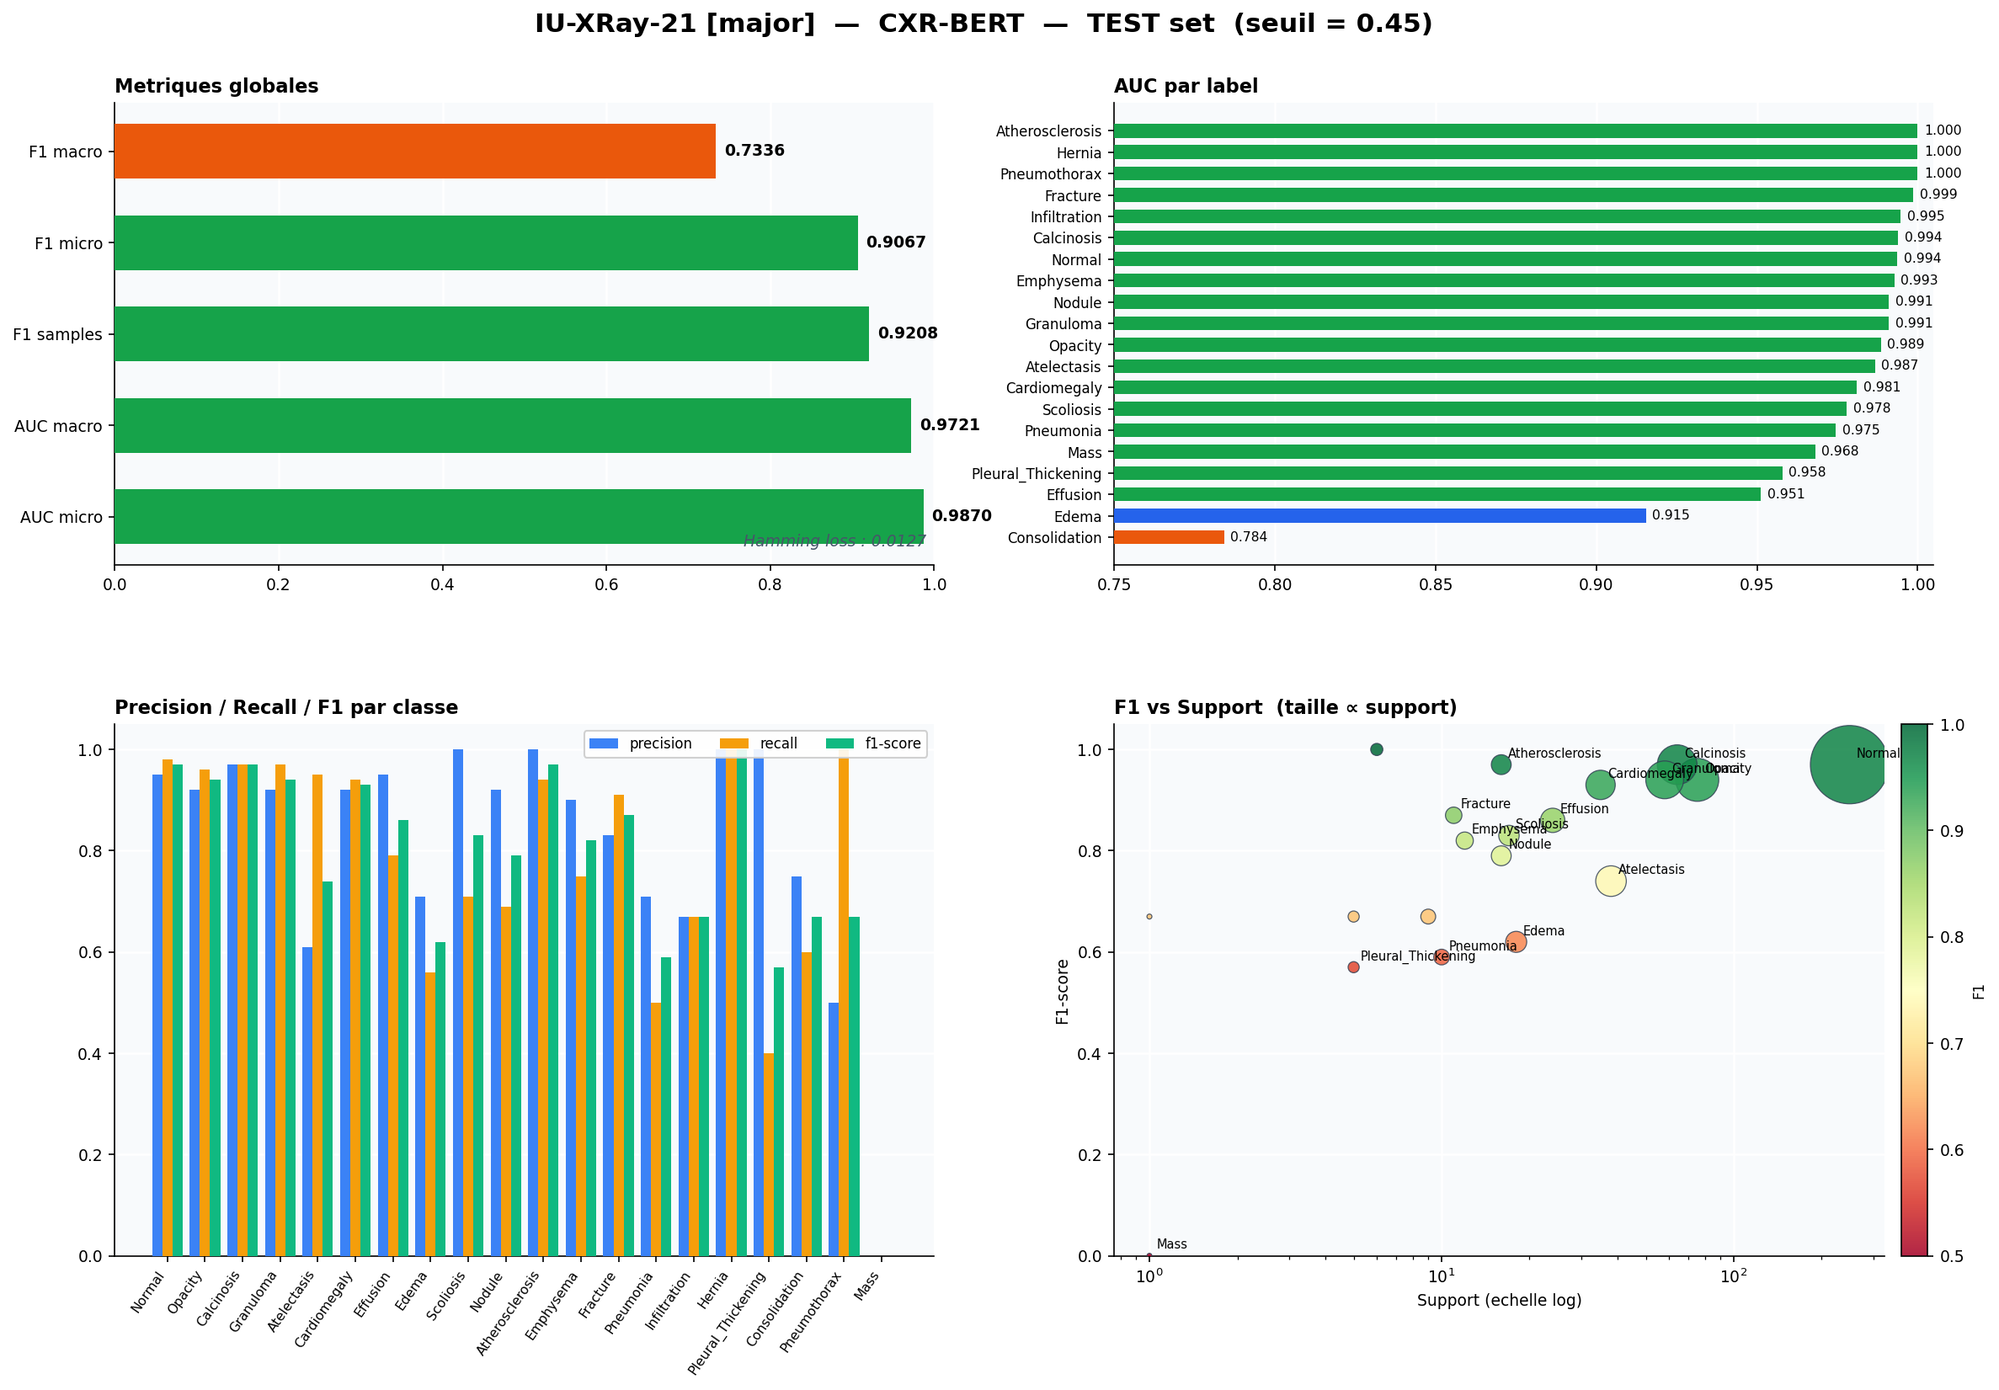
\includegraphics[width=\linewidth]{figures/cxrbert_test.png}\caption{CXR-BERT-specialized -- 21-label test.}\end{subfigure}
\caption{Text-only classifiers: a bag-of-words baseline is already strong; CXR-BERT is near-saturated.}
\end{figure}

% ============================================================
\section{Image (A.\,Chebil)}
% ============================================================
\footnotesize
Image-only models plateau much lower. \textbf{DenseNet-121} (ImageNet, BCE) reaches
mean AUC \textbf{0.78} (some overfit); a \textbf{ViT} (\texttt{vit-chest-xray}) with
Asymmetric Loss and strong augmentation reaches \textbf{0.733} without overfit. The
gap to text confirms how much label signal the report carries.

\begin{figure}[H]
\centering
\begin{subfigure}{0.32\textwidth}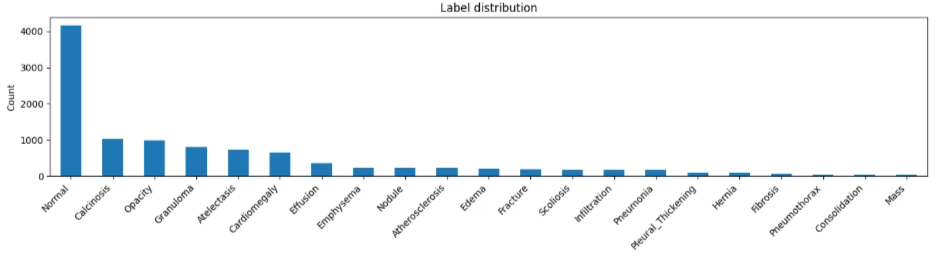
\includegraphics[width=\linewidth]{figures/dataset.png}\caption{Label distribution.}\end{subfigure}
\hfill
\begin{subfigure}{0.32\textwidth}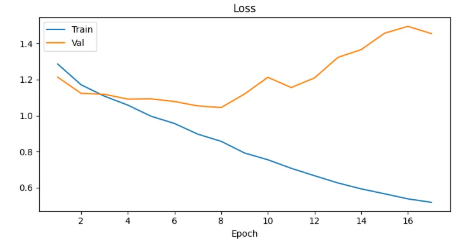
\includegraphics[width=\linewidth]{figures/densenet_loss_func.png}\caption{DenseNet-121 loss.}\end{subfigure}
\hfill
\begin{subfigure}{0.32\textwidth}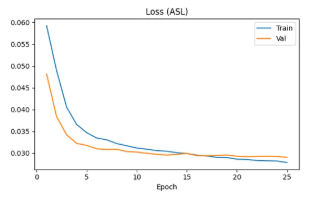
\includegraphics[width=\linewidth]{figures/ViT_final_loss_func.png}\caption{ViT loss (ASL).}\end{subfigure}
\caption{Imbalanced labels (a) and image-only training (b--c).}
\end{figure}

% ============================================================
\section{Multimodal Fusion}
% ============================================================
\footnotesize
\textbf{Architecture~1 -- bidirectional cross-attention (A.\,Chebil).} A custom text
encoder and the ViT are projected to $d{=}512$; text$\to$image (t2i) and
image$\to$text (i2t) cross-attentions run in parallel, pooled, concatenated and
classified. Two-phase training (frozen warmup then full unfreeze, Asymmetric Loss)
reaches mean test AUC \textbf{0.9886} (21 labels). A \emph{cross-modal mediation}
study, however, shows this gain is largely \emph{text leakage}: dropping the report
while keeping an i2t-shaped image representation costs $\approx$0 AUC.

\begin{table}[H]
\centering\footnotesize
\caption{Mediation -- mean AUC over 21 pathologies ($n=968$). Image-with-i2t carries the signal.}
\begin{tabular}{cccc}
\toprule
real\_real (full) & blankT+realI & realT+blankI & $\Delta$(real$-$blankT+realI) \\
\midrule
0.9833 & 0.9824 & 0.7648 & $+0.0010$ \\
\bottomrule
\end{tabular}
\end{table}

\textbf{Architecture~3 -- Q-Former (H.\,Hennion).} Both encoders \emph{frozen}; 14
learnable label-queries are distilled through 3 Joint Query Blocks (self-attn on
$[Q;T]$, cross-attn $Q\!\to\!$image, FFN) into a diagonal label-aligned head
($\sim$28--31M trainable). The \textbf{last} variant reads the final CXR-BERT layer
(macro AUC \textbf{0.974}); the \textbf{deep} variant taps layers 10/11/12
coarse$\to$fine (\textbf{0.978}) -- above the image baselines and on par with text.

\emph{Explainability \& modality balance.} Frozen-encoder queries suffer
\textbf{collapse} (effective rank $13\!\to\!1.5$), the mechanism behind text
dominance. \textbf{Pre-norm} is a clear jump (macro AUC \textbf{0.9836}); modality
(text) dropout + reinject (\texttt{variant\_c}, \textbf{0.9795}) and an
attention-pooled head trade a little accuracy for far more localised, label-specific
attention; \textbf{CGGM} re-balances the streams by pulling the fusion head toward
the lagging modality. Probing \emph{unimodality} (\texttt{--no\_findings}: infer on
indication + image only) drops to macro AUC \textbf{0.698} -- promising but not yet
conclusive.

\begin{figure}[H]
\centering
\begin{subfigure}{0.62\textwidth}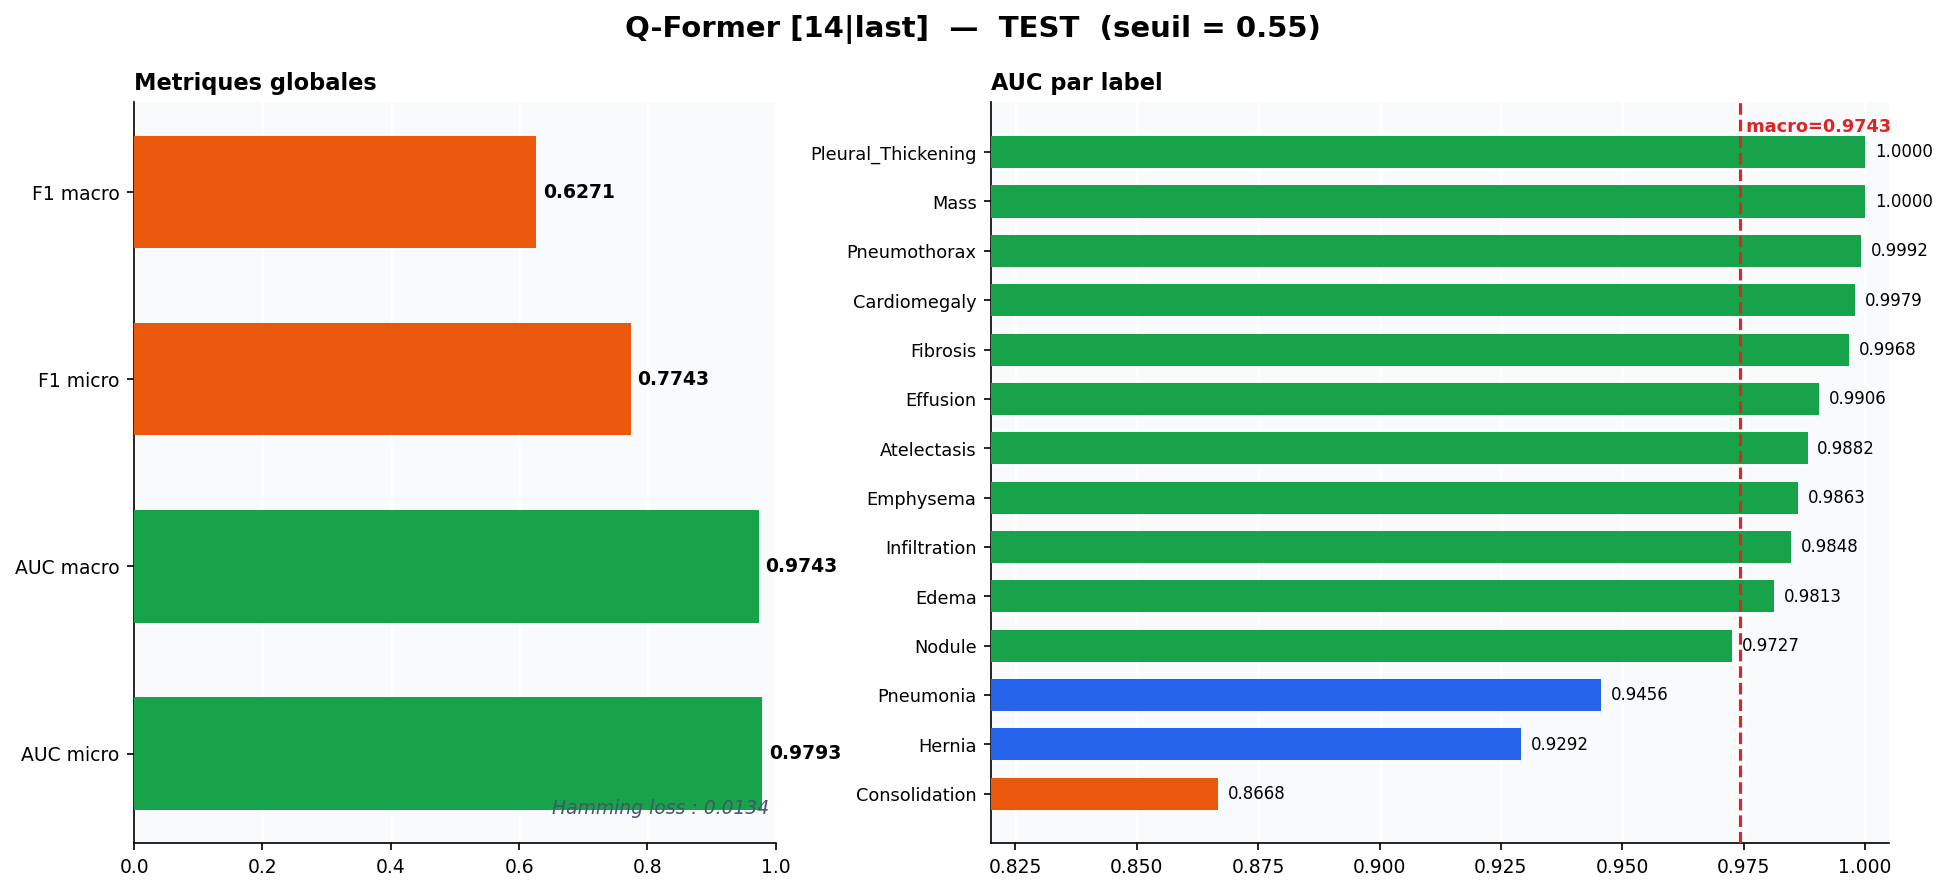
\includegraphics[width=\linewidth]{figures/qformer_last_test.png}\caption{Q-Former [last] -- test metrics \& per-label AUC.}\end{subfigure}
\hfill
\begin{subfigure}{0.36\textwidth}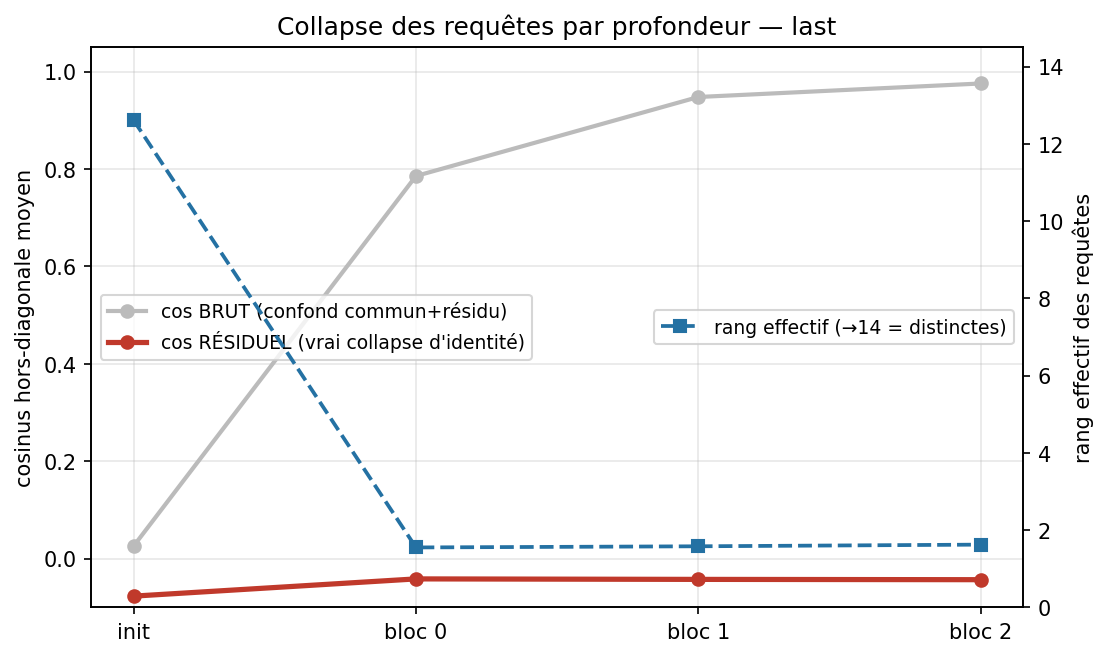
\includegraphics[width=\linewidth]{figures/qformer_collapse.png}\caption{Query collapse (rank $\to$1) motivates anti-collapse.}\end{subfigure}
\\[3pt]
\begin{subfigure}{0.62\textwidth}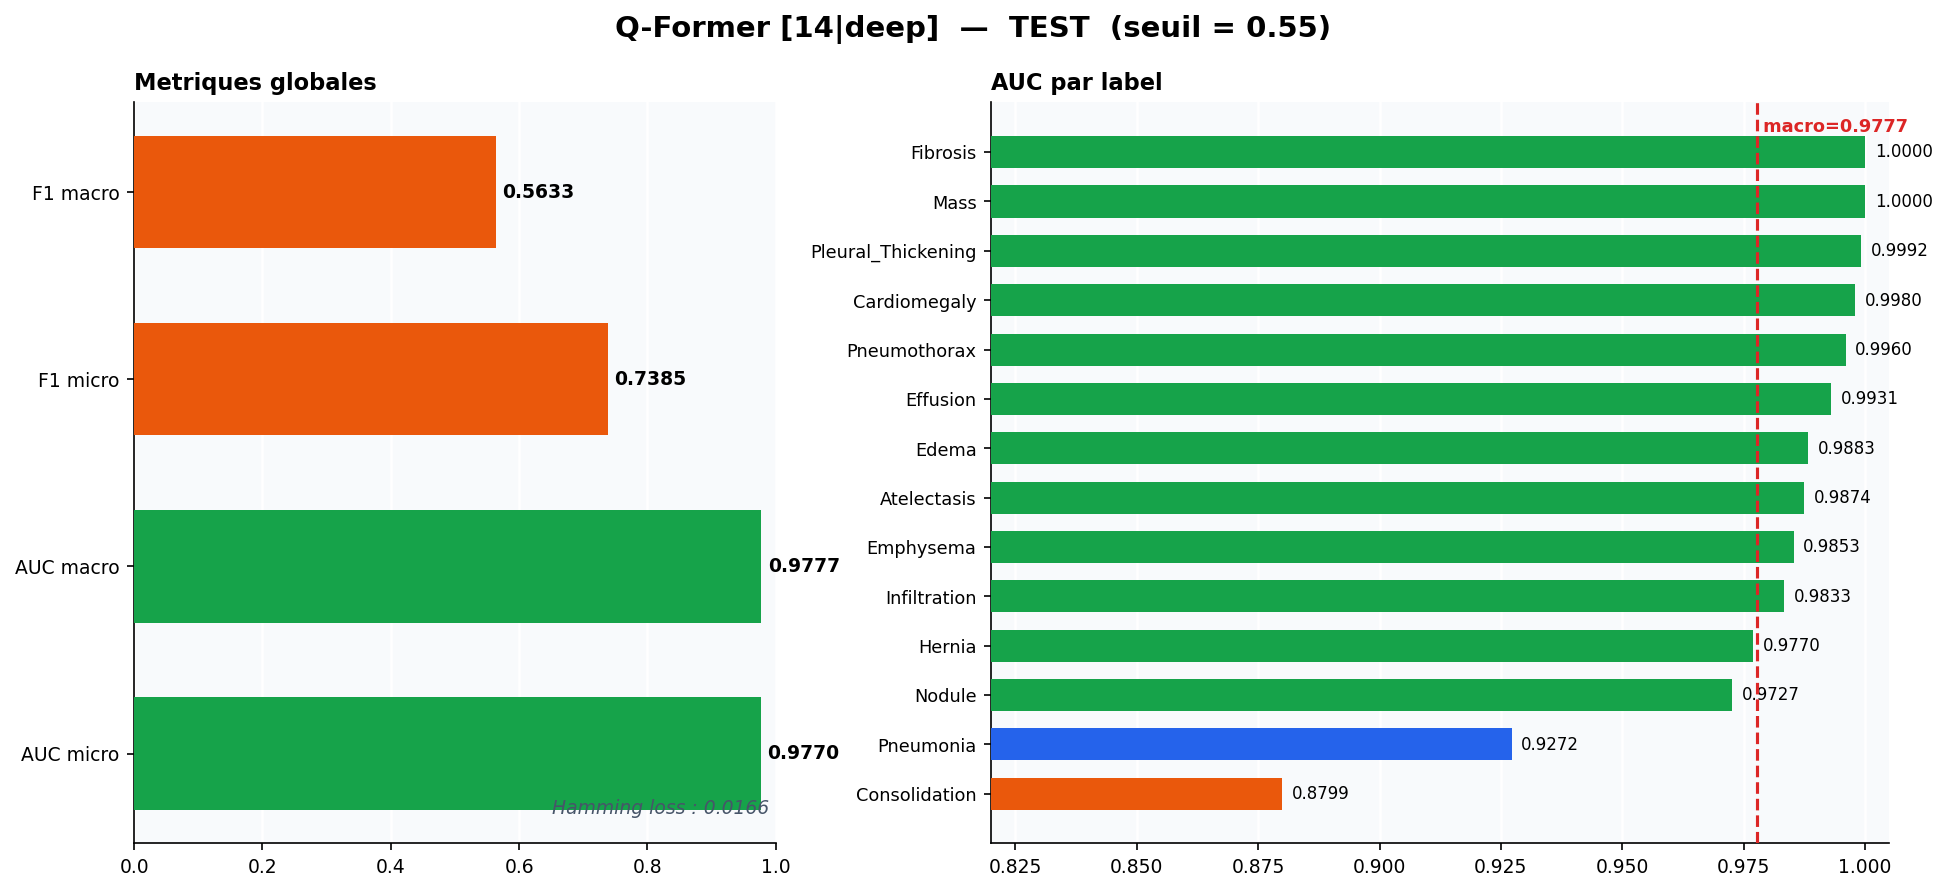
\includegraphics[width=\linewidth]{figures/qformer_deep_test.png}\caption{Q-Former [deep] -- test metrics \& per-label AUC.}\end{subfigure}
\hfill
\begin{subfigure}{0.36\textwidth}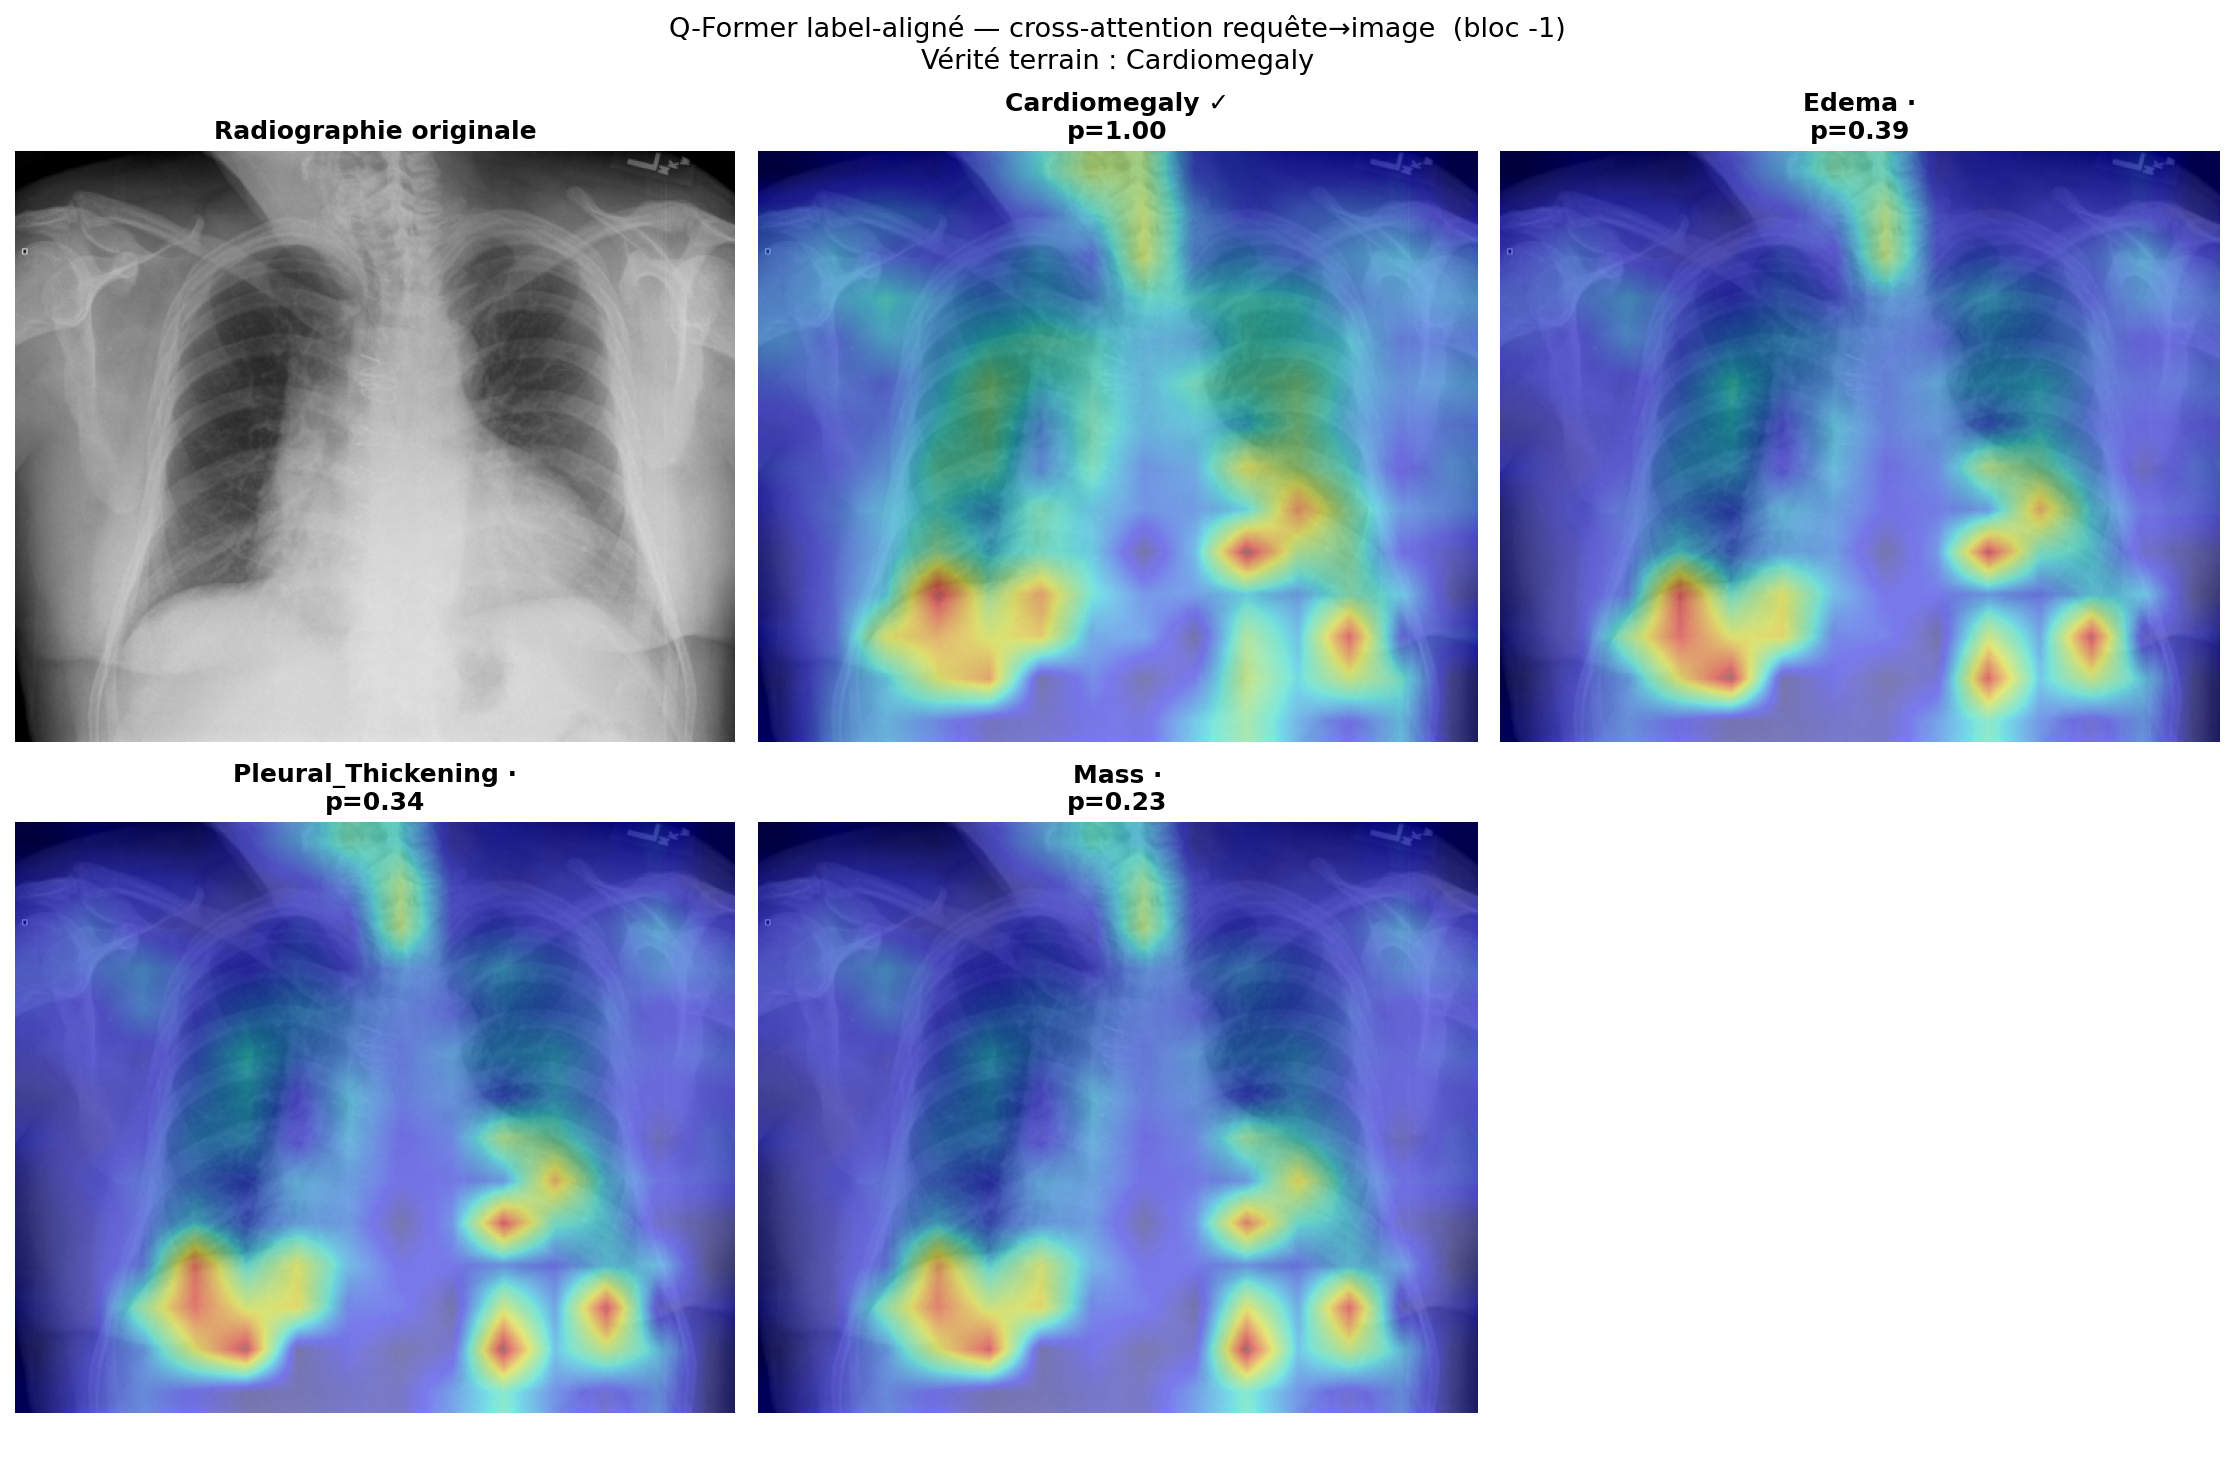
\includegraphics[width=\linewidth]{figures/qformer_variantC_attention.png}\caption{\texttt{variant\_c}: label-aligned attention, Cardiomegaly.}\end{subfigure}
\caption{Q-Former results (last/deep), query collapse, and interpretable per-label cross-attention.}
\end{figure}

\noindent\footnotesize\textbf{Takeaway.} Text alone is strong, image alone weak;
fusion improves over vision but is largely text-mediated. Interpretability work
(\texttt{variant\_c}, CGGM, attention-pooled head) trades a little accuracy for a
more trustworthy, less text-dominated model; unimodal indication\,+\,image is the
open problem.

\end{document}
